\documentclass[12pt,a4paper]{article}
\usepackage[utf8]{inputenc}
\usepackage[T1]{fontenc}
\usepackage{tikz}
\usepackage{geometry}
\usetikzlibrary{shapes.multipart, arrows, positioning, fit, calc}

\geometry{landscape, margin=1cm}

\begin{document}

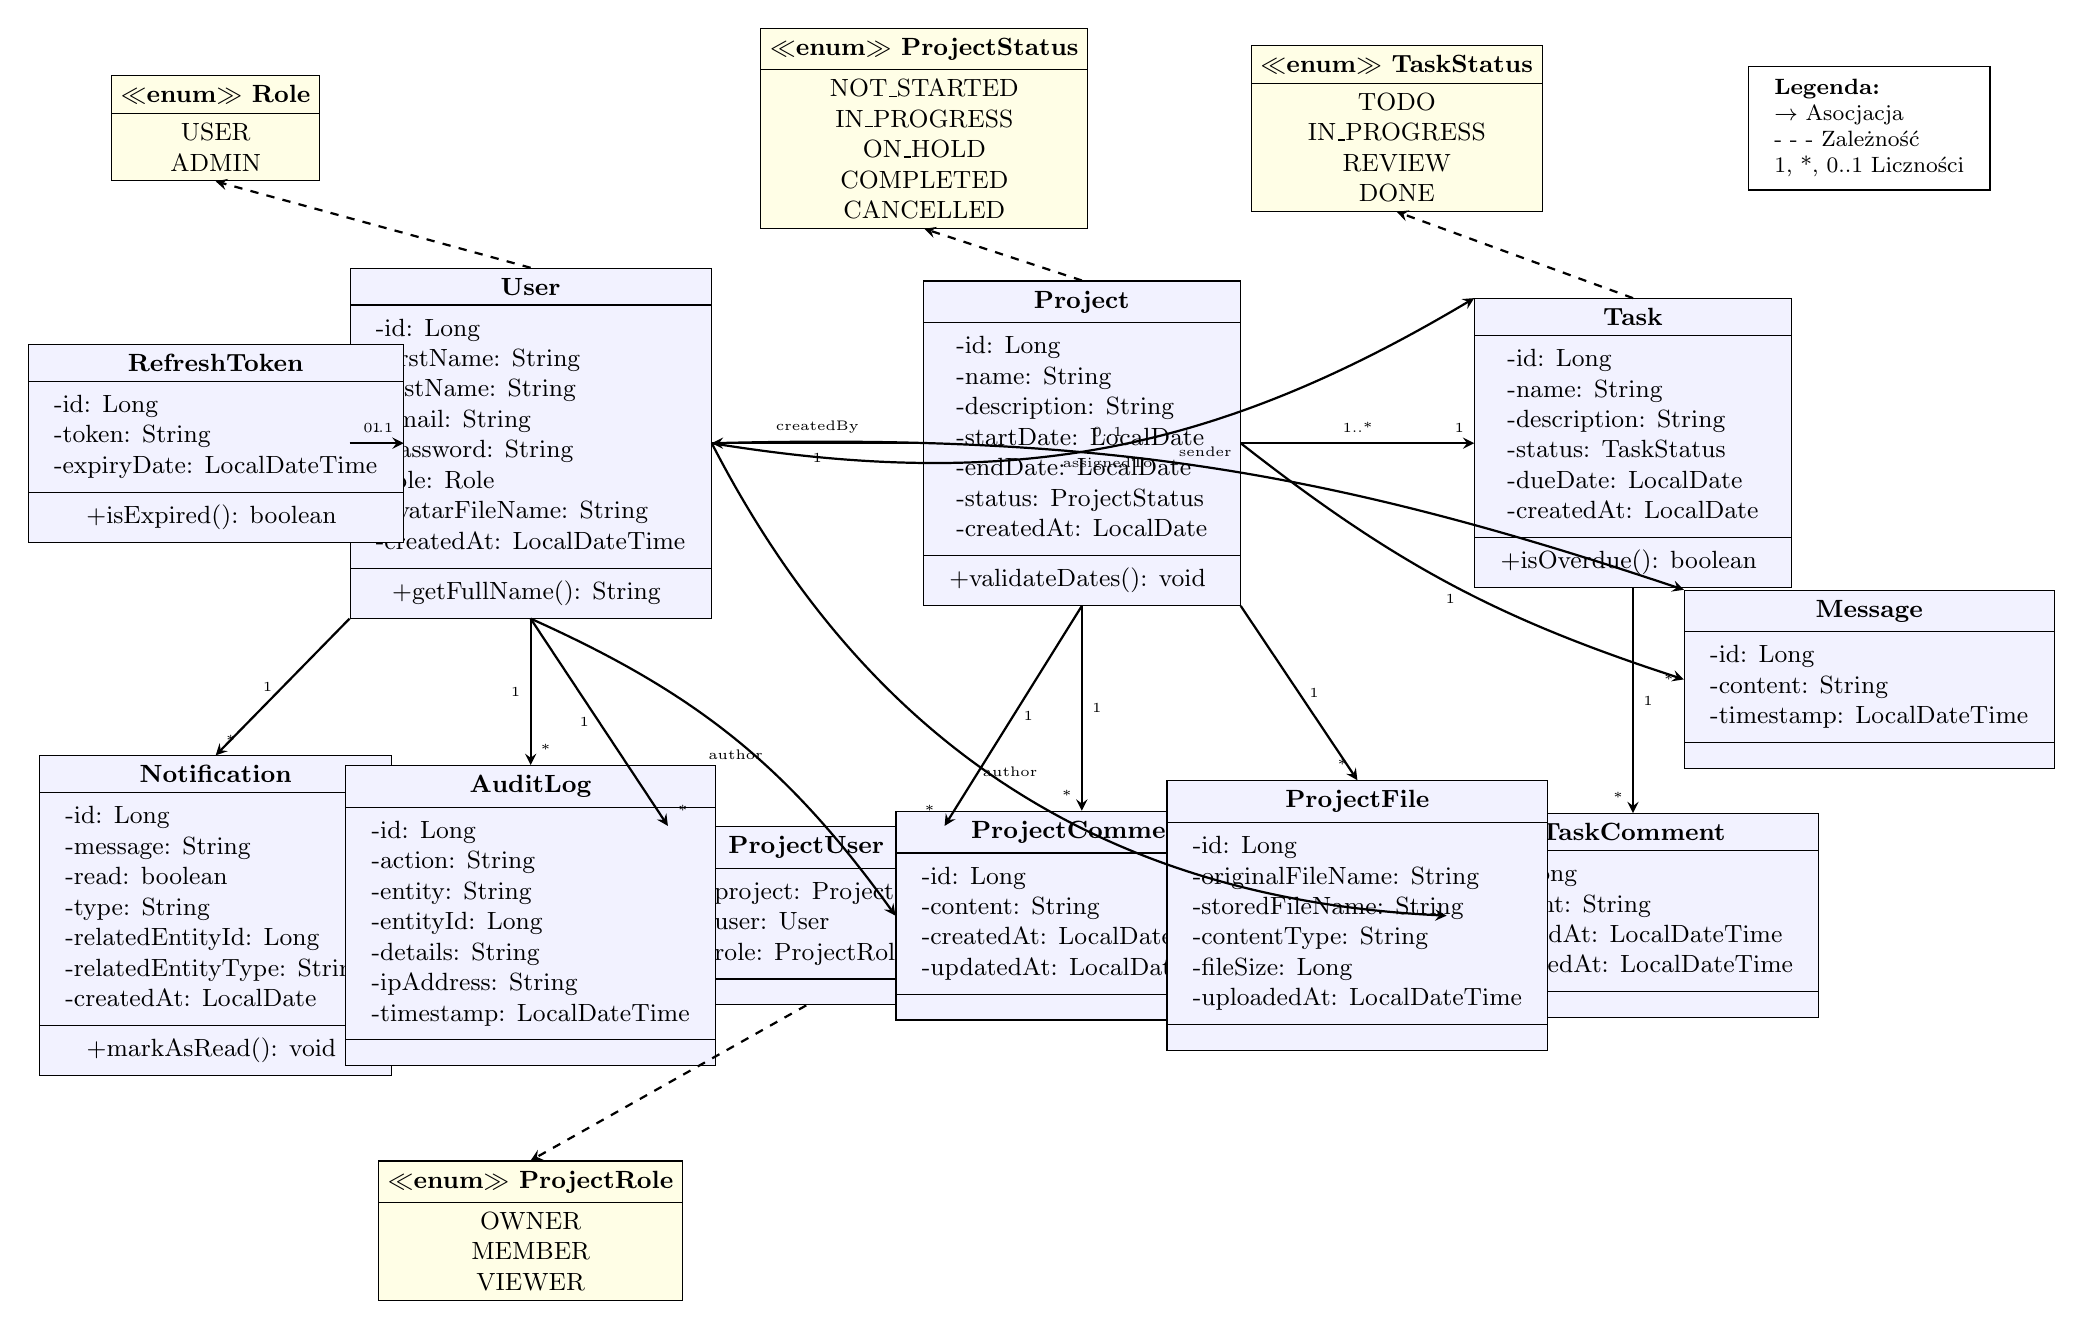
\begin{tikzpicture}[
    class/.style={
        rectangle split,
        rectangle split parts=3,
        draw,
        fill=blue!5,
        minimum width=3.5cm,
        font=\small,
        align=center
    },
    enum/.style={
        rectangle split,
        rectangle split parts=2,
        draw,
        fill=yellow!10,
        minimum width=2.5cm,
        font=\small,
        align=center
    },
    association/.style={->, >=stealth, thick},
    composition/.style={->, >=stealth, thick, 
        decoration={markings, mark=at position 0 with 
            {\fill (0,0) -- (2mm,1.5mm) -- (4mm,0) -- (2mm,-1.5mm) -- cycle;}},
        postaction={decorate}
    },
    aggregation/.style={->, >=stealth, thick,
        decoration={markings, mark=at position 0 with 
            {\draw (0,0) -- (2mm,1.5mm) -- (4mm,0) -- (2mm,-1.5mm) -- cycle;}},
        postaction={decorate}
    }
]

% =====================
% ENCJE GŁÓWNE
% =====================

% User
\node[class] (user) at (0,0) {
    \textbf{User}
    \nodepart{second}
    \begin{tabular}{l}
    -id: Long \\
    -firstName: String \\
    -lastName: String \\
    -email: String \\
    -password: String \\
    -role: Role \\
    -avatarFileName: String \\
    -createdAt: LocalDateTime
    \end{tabular}
    \nodepart{third}
    \begin{tabular}{l}
    +getFullName(): String
    \end{tabular}
};

% Project
\node[class] (project) at (7,0) {
    \textbf{Project}
    \nodepart{second}
    \begin{tabular}{l}
    -id: Long \\
    -name: String \\
    -description: String \\
    -startDate: LocalDate \\
    -endDate: LocalDate \\
    -status: ProjectStatus \\
    -createdAt: LocalDate
    \end{tabular}
    \nodepart{third}
    \begin{tabular}{l}
    +validateDates(): void
    \end{tabular}
};

% Task
\node[class] (task) at (14,0) {
    \textbf{Task}
    \nodepart{second}
    \begin{tabular}{l}
    -id: Long \\
    -name: String \\
    -description: String \\
    -status: TaskStatus \\
    -dueDate: LocalDate \\
    -createdAt: LocalDate
    \end{tabular}
    \nodepart{third}
    \begin{tabular}{l}
    +isOverdue(): boolean
    \end{tabular}
};

% ProjectUser (tabela łącząca)
\node[class] (projectuser) at (3.5,-6) {
    \textbf{ProjectUser}
    \nodepart{second}
    \begin{tabular}{l}
    -project: Project \\
    -user: User \\
    -role: ProjectRole
    \end{tabular}
    \nodepart{third}
    \begin{tabular}{l}
    \end{tabular}
};

% ProjectComment
\node[class] (pcomment) at (7,-6) {
    \textbf{ProjectComment}
    \nodepart{second}
    \begin{tabular}{l}
    -id: Long \\
    -content: String \\
    -createdAt: LocalDateTime \\
    -updatedAt: LocalDateTime
    \end{tabular}
    \nodepart{third}
    \begin{tabular}{l}
    \end{tabular}
};

% TaskComment
\node[class] (tcomment) at (14,-6) {
    \textbf{TaskComment}
    \nodepart{second}
    \begin{tabular}{l}
    -id: Long \\
    -content: String \\
    -createdAt: LocalDateTime \\
    -updatedAt: LocalDateTime
    \end{tabular}
    \nodepart{third}
    \begin{tabular}{l}
    \end{tabular}
};

% ProjectFile
\node[class] (pfile) at (10.5,-6) {
    \textbf{ProjectFile}
    \nodepart{second}
    \begin{tabular}{l}
    -id: Long \\
    -originalFileName: String \\
    -storedFileName: String \\
    -contentType: String \\
    -fileSize: Long \\
    -uploadedAt: LocalDateTime
    \end{tabular}
    \nodepart{third}
    \begin{tabular}{l}
    \end{tabular}
};

% Notification
\node[class] (notification) at (-4,-6) {
    \textbf{Notification}
    \nodepart{second}
    \begin{tabular}{l}
    -id: Long \\
    -message: String \\
    -read: boolean \\
    -type: String \\
    -relatedEntityId: Long \\
    -relatedEntityType: String \\
    -createdAt: LocalDate
    \end{tabular}
    \nodepart{third}
    \begin{tabular}{l}
    +markAsRead(): void
    \end{tabular}
};

% AuditLog
\node[class] (auditlog) at (0,-6) {
    \textbf{AuditLog}
    \nodepart{second}
    \begin{tabular}{l}
    -id: Long \\
    -action: String \\
    -entity: String \\
    -entityId: Long \\
    -details: String \\
    -ipAddress: String \\
    -timestamp: LocalDateTime
    \end{tabular}
    \nodepart{third}
    \begin{tabular}{l}
    \end{tabular}
};

% Message (Chat)
\node[class] (message) at (17,-3) {
    \textbf{Message}
    \nodepart{second}
    \begin{tabular}{l}
    -id: Long \\
    -content: String \\
    -timestamp: LocalDateTime
    \end{tabular}
    \nodepart{third}
    \begin{tabular}{l}
    \end{tabular}
};

% RefreshToken
\node[class] (token) at (-4,0) {
    \textbf{RefreshToken}
    \nodepart{second}
    \begin{tabular}{l}
    -id: Long \\
    -token: String \\
    -expiryDate: LocalDateTime
    \end{tabular}
    \nodepart{third}
    \begin{tabular}{l}
    +isExpired(): boolean
    \end{tabular}
};

% =====================
% ENUMY
% =====================

% Role
\node[enum] (role) at (-4,4) {
    \textbf{$\ll$enum$\gg$ Role}
    \nodepart{second}
    USER\\ADMIN
};

% ProjectStatus
\node[enum] (pstatus) at (5,4) {
    \textbf{$\ll$enum$\gg$ ProjectStatus}
    \nodepart{second}
    NOT\_STARTED\\IN\_PROGRESS\\ON\_HOLD\\COMPLETED\\CANCELLED
};

% TaskStatus
\node[enum] (tstatus) at (11,4) {
    \textbf{$\ll$enum$\gg$ TaskStatus}
    \nodepart{second}
    TODO\\IN\_PROGRESS\\REVIEW\\DONE
};

% ProjectRole
\node[enum] (prole) at (0,-10) {
    \textbf{$\ll$enum$\gg$ ProjectRole}
    \nodepart{second}
    OWNER\\MEMBER\\VIEWER
};

% =====================
% RELACJE
% =====================

% User -> Role
\draw[association, dashed] (user.north) -- (role.south);

% Project -> ProjectStatus
\draw[association, dashed] (project.north) -- (pstatus.south);

% Task -> TaskStatus
\draw[association, dashed] (task.north) -- (tstatus.south);

% ProjectUser -> ProjectRole
\draw[association, dashed] (projectuser.south) -- (prole.north);

% User <-> Project (Many-to-Many through ProjectUser)
\draw[association] (user.south) -- node[left, font=\tiny] {1} 
    (projectuser.north west) node[above right, font=\tiny] {*};
\draw[association] (project.south) -- node[right, font=\tiny] {1} 
    (projectuser.north east) node[above left, font=\tiny] {*};

% Project -> Task (One-to-Many)
\draw[association] (project.east) -- node[above, font=\tiny] {1..*} (task.west)
    node[above left, font=\tiny] {1};

% User -> Task (assigned)
\draw[association, bend right=20] (user.east) to node[above, font=\tiny] {0..1} 
    node[below, font=\tiny] {assignedTo} (task.north west);

% Project -> createdBy (User)
\draw[association] (project.west) -- node[above, font=\tiny] {createdBy} 
    node[below, font=\tiny] {1} (user.east);

% User -> Notification (One-to-Many)
\draw[association] (user.south west) -- node[left, font=\tiny] {1} 
    (notification.north) node[above right, font=\tiny] {*};

% User -> AuditLog (One-to-Many)
\draw[association] (user.south) -- node[left, font=\tiny] {1} 
    (auditlog.north) node[above right, font=\tiny] {*};

% User -> RefreshToken
\draw[association] (user.west) -- node[above, font=\tiny] {1} 
    (token.east) node[above left, font=\tiny] {0..1};

% Project -> ProjectComment
\draw[association] (project.south) -- node[right, font=\tiny] {1} 
    (pcomment.north) node[above left, font=\tiny] {*};

% Project -> ProjectFile
\draw[association] (project.south east) -- node[right, font=\tiny] {1} 
    (pfile.north) node[above left, font=\tiny] {*};

% Task -> TaskComment
\draw[association] (task.south) -- node[right, font=\tiny] {1} 
    (tcomment.north) node[above left, font=\tiny] {*};

% User -> ProjectComment (author)
\draw[association, bend left=15] (user.south) to 
    node[below, font=\tiny] {author} (pcomment.west);

% User -> TaskComment (author)
\draw[association, bend right=30] (user.east) to 
    node[above, font=\tiny] {author} (tcomment.west);

% User -> Message (sender)
\draw[association] (user.east) to[bend left=10] 
    node[above, font=\tiny] {sender} (message.north west);

% Project -> Message
\draw[association] (project.east) to[bend right=10] 
    node[below, font=\tiny] {1} (message.west) node[left, font=\tiny] {*};

% Legenda
\node[draw, fill=white, font=\footnotesize] at (17,4) {
    \begin{tabular}{l}
    \textbf{Legenda:}\\
    $\rightarrow$ Asocjacja\\
    - - - Zależność\\
    1, *, 0..1 Liczności
    \end{tabular}
};

\end{tikzpicture}

\end{document}
